\chapter{System Design and RISC-V Platform}
\label{ch:platform}

\section{Deployment Context and Platform Overview}

The implemented design targets the Terasic DE1-SoC development board, which
carries a Cyclone~V 5CSEMA5F31C6 FPGA device~\citep{de1soc_manual}. The SoC
is synthesised entirely into the FPGA fabric; it does not use the hard ARM
Cortex-A9 processor on the DE1-SoC's HPS. This choice keeps the design
self-contained in the FPGA, makes cycle-level timing directly controllable
through HDL, and avoids the complexity of AXI bridges, Linux boot, and HPS
memory management.

The entire benchmark path executes on-chip: firmware, CSR arrays, dense matrix
$B$, and output matrix $C$ all reside in the shared 64\,KB dual-port block RAM.
This simplifies the memory system and makes cycle comparisons easier to interpret
at the cost of limiting the benchmark problem sizes to those that fit comfortably
in on-chip memory. The design runs from the 50\,MHz on-board oscillator.

Figure~\ref{fig:soc-block} shows the top-level block diagram of the implemented
SoC.

\begin{figure}[htbp]
    \centering
    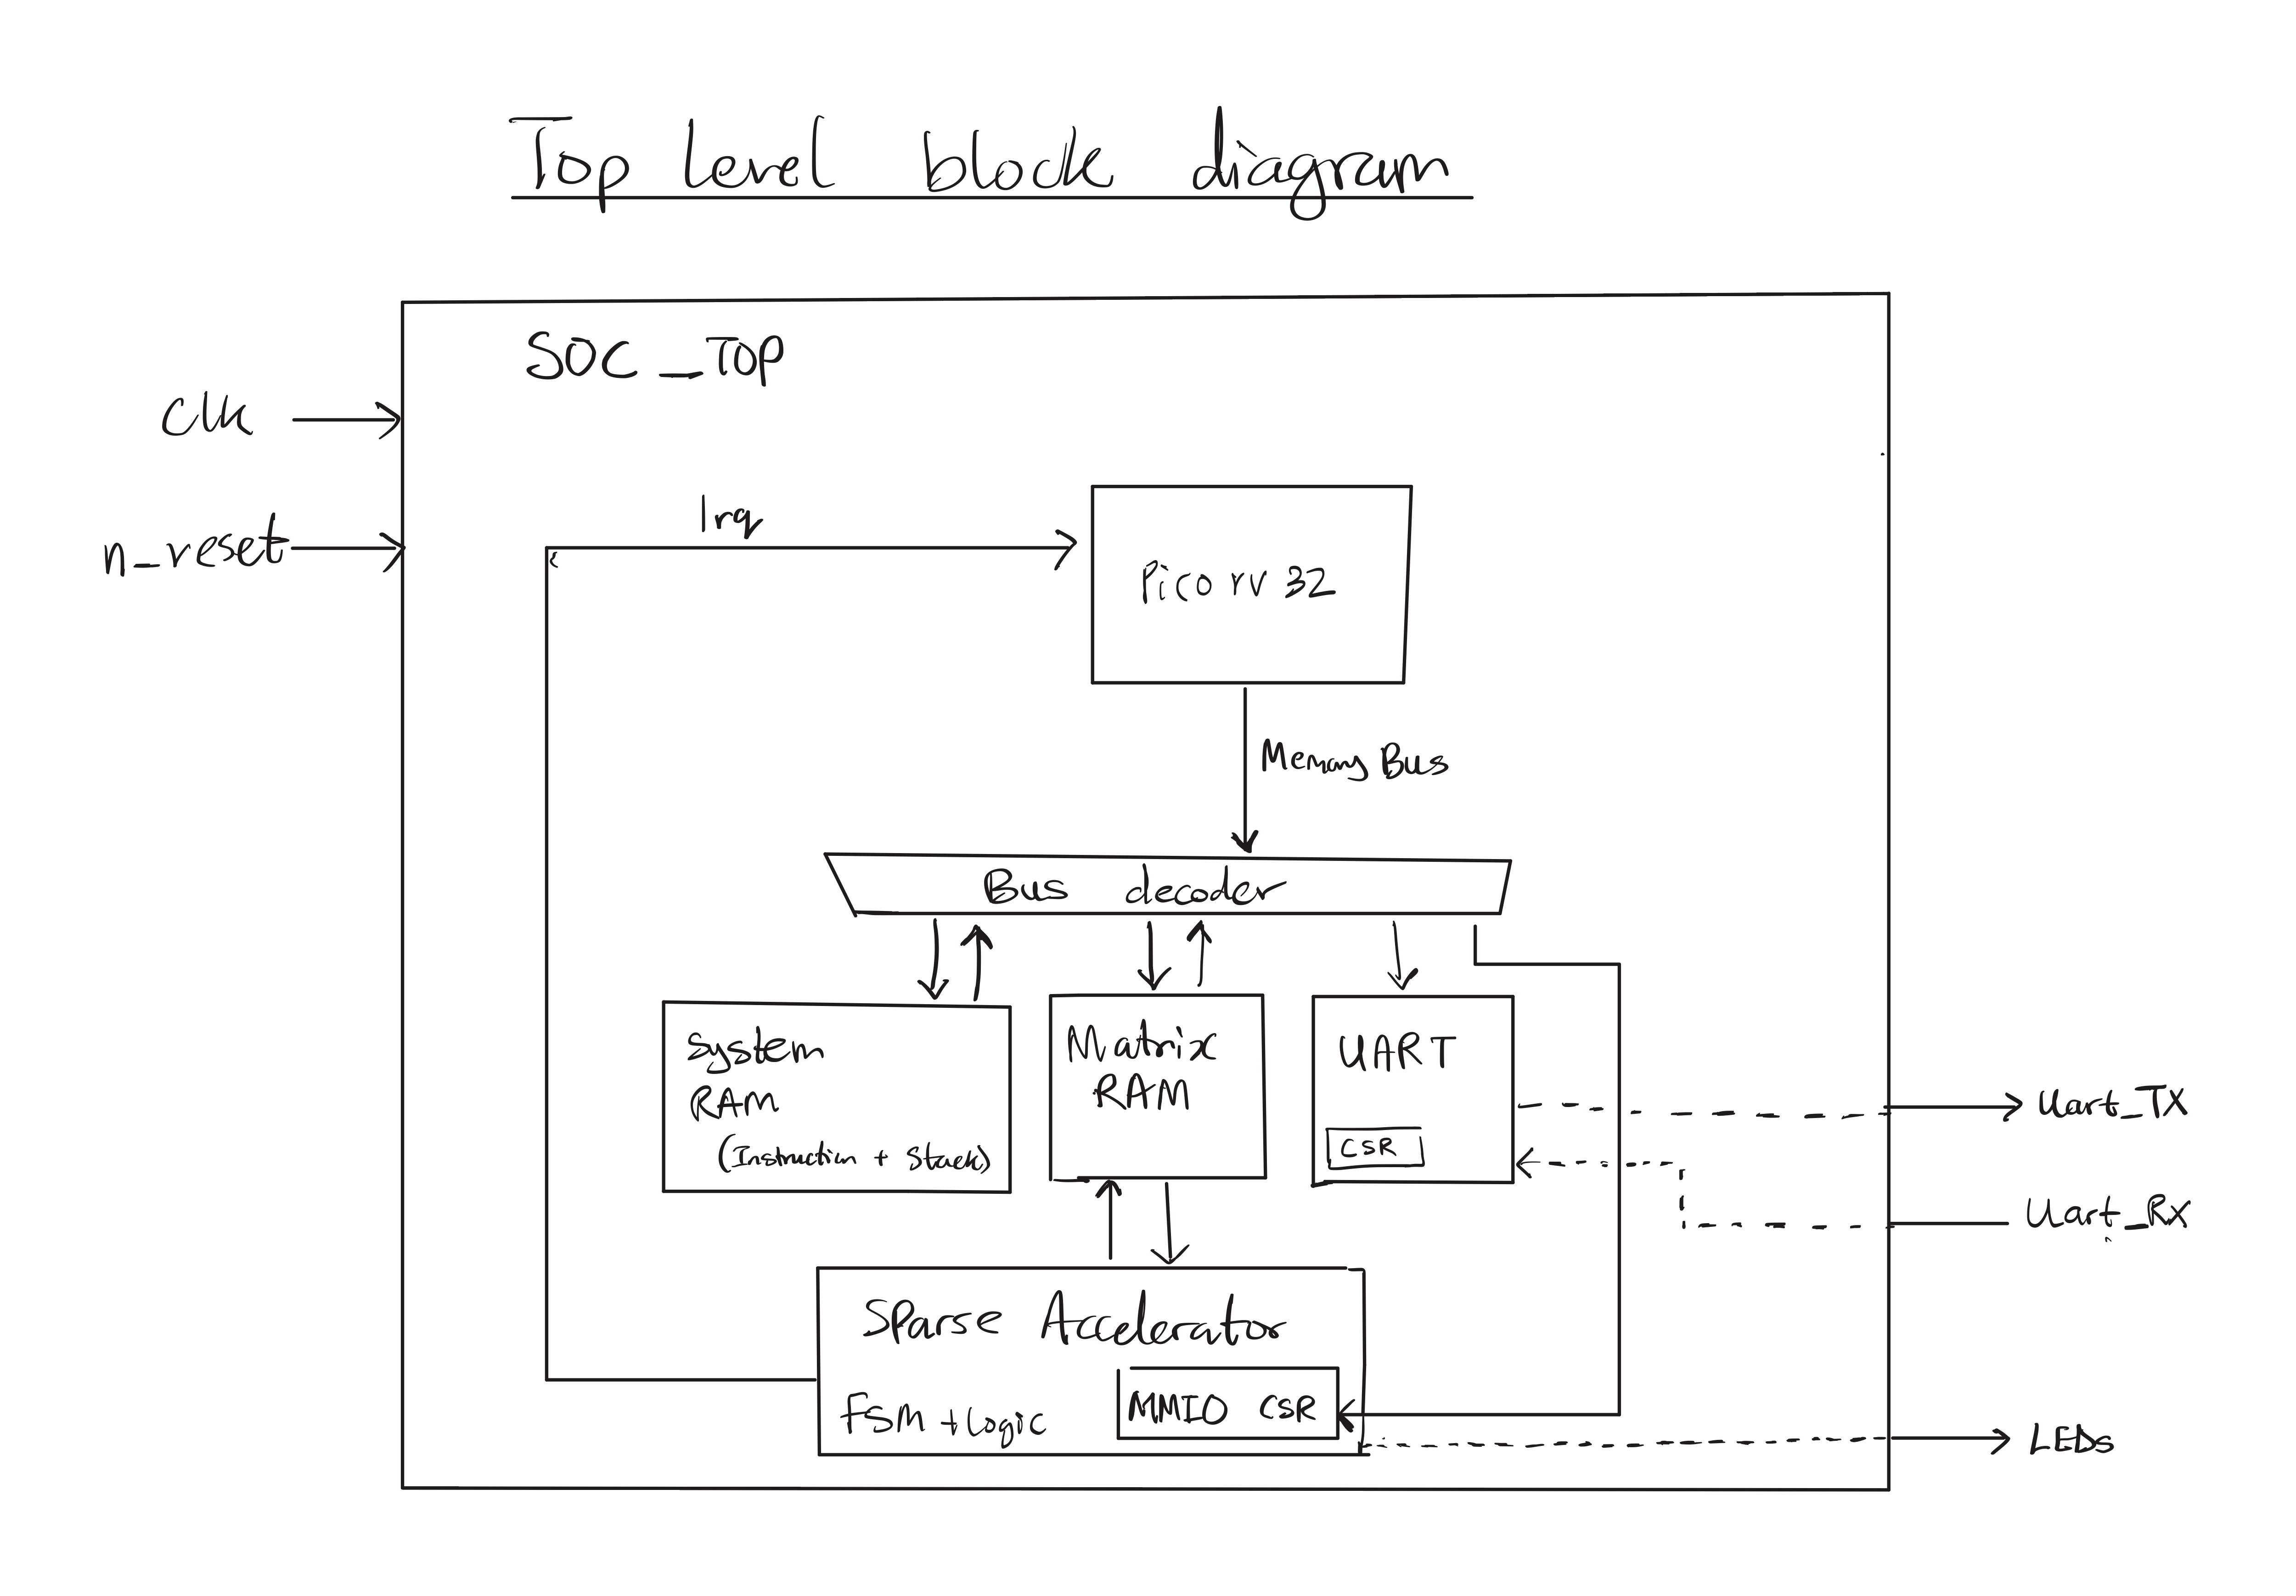
\includegraphics[width=1\textwidth]{top_block_dia.jpg}
    \caption{Top-level RISC-V SoC block diagram showing PicoRV32 CPU, shared
             dual-port RAM, SpMM accelerator, UART peripheral, and GPIO
             interface, all connected via memory-mapped I/O.}
    \label{fig:soc-block}
\end{figure}

\section{Target FPGA: Cyclone V Resources}

The Cyclone~V 5CSEMA5F31C6 device provides the following key resources
\citep{cyclonev_handbook}:

\begin{table}[htbp]
  \centering
  \small
  \begin{tabular}{lrr}
  \toprule
  Resource & Total available & Used (estimated) \\
  \midrule
  Adaptive Logic Modules (ALMs) & 32,070 & $\approx$5,000 (16\%) \\
  Logic registers & 128,280 & $\approx$8,000 (6\%) \\
  M10K memory blocks (10\,Kbit each) & 397 & $\approx$20 (5\%) \\
  DSP 18$\times$18 multiplier blocks & 87 & $\approx$8 (9\%) \\
  I/O pins & 457 & --- \\
  \bottomrule
  \end{tabular}
  \caption{Cyclone~V 5CSEMA5F31C6 resource availability and estimated
           design utilisation. Final synthesis numbers are pending completion
           of the Quartus timing closure study.}
  \label{tab:fpga-resources}
\end{table}

The M10K blocks each provide 10\,Kbits (approximately 1.25\,KB) of configurable
on-chip memory~\citep{intel_m10k}. At true-dual-port configuration with
32-bit-wide ports, each M10K can hold 256 words. The 64\,KB BRAM used in this
design requires approximately 16 M10K blocks in a cascaded configuration, leaving
substantial BRAM capacity for other purposes. The DSP blocks implement
18$\times$18-bit two's-complement signed multipliers followed by a dedicated
accumulator register, making them well-suited to INT32 MAC operations when
configured appropriately~\citep{intel_dsp_blocks}.

\section{PicoRV32 Host Processor}

The host processor is PicoRV32~\citep{picorv32}, a compact RV32IM soft-core
implementing the RISC-V base integer instruction set with the hardware integer
multiply extension (M)~\citep{riscv_isa}. PicoRV32 was chosen because:
\begin{itemize}
  \item it is small (approximately 700--1000 ALMs), leaving adequate FPGA fabric
        for the accelerator and memory;
  \item it supports the \texttt{rdcycle} performance counter CSR natively, which
        is used for all cycle-accurate timing measurements; and
  \item it exposes a simple memory bus (valid/ready handshake with address, data,
        and write-enable signals) that maps directly onto the SoC interconnect.
\end{itemize}

PicoRV32 is an in-order, non-pipelined core. It issues one instruction at a time,
incurring full stall cycles on every load instruction. For instructions that access
the synchronous dual-port BRAM, the latency is one clock cycle after the address
is presented. This is important for interpreting accelerator speedups: the CPU
software baseline is a simple in-order core with no caching and no out-of-order
execution, making the accelerator's advantage larger than it would be against a
modern superscalar CPU.

The M extension provides hardware 32$\times$32 integer multiply and divide. The
software SpMM reference uses \texttt{MUL} instructions for the inner-loop
multiply--accumulate. Without the M extension, PicoRV32 would fall back to a
software multiply routine that is typically 10--30$\times$ slower, which would
artificially inflate speedup numbers. The M extension is therefore required for
a credible software baseline.

\section{System Memory Map and Bus Architecture}

\subsection{Bus Protocol}

The SoC interconnect uses the native PicoRV32 memory bus: a
valid/ready handshake with a 32-bit address bus, a 32-bit bidirectional data
bus, a 4-bit byte-enable signal, and a read/write indicator. The bus is
synchronous to the 50\,MHz system clock. Access latency is a single cycle for
BRAM (using the BRAM's registered output) and combinatorial for MMIO registers.

\subsection{Address Space}

Table~\ref{tab:system-memory-map} summarises the complete system memory map.

\begin{table}[htbp]
  \centering
  \small
  \begin{tabular}{lp{3.0cm}p{5.5cm}}
  \toprule
  Address range & Peripheral & Purpose \\
  \midrule
  \texttt{0x0000\_0000--0x0000\_FFFF} & On-chip RAM (64\,KB) &
    Firmware code, stack, CSR arrays (\texttt{rowptr}, \texttt{colidx},
    \texttt{values}), dense matrix $B$, output matrix $C$ \\[4pt]
  \texttt{0x1000\_0000--0x1000\_00FF} & SpMM accelerator MMIO &
    Configuration registers, control, and status \\[4pt]
  \texttt{0x2000\_0000--0x2000\_000F} & GPIO &
    LED output, switch and button input, seven-segment display \\[4pt]
  \texttt{0x2000\_0100--0x2000\_01FF} & UART (\texttt{simpleuart}) &
    Serial output for UART benchmark reporting at 115200\,baud \\
  \bottomrule
  \end{tabular}
  \caption{System memory map of the implemented RISC-V SoC.}
  \label{tab:system-memory-map}
\end{table}

\subsection{Dual-Port BRAM Organisation}

The 64\,KB on-chip RAM is implemented as an Altera \texttt{altsyncram}
true-dual-port memory with 32-bit-wide ports. Port~A is connected exclusively
to the PicoRV32 CPU and supports byte-granular write-enable (4-bit byte
mask). Port~B is connected exclusively to the SpMM accelerator and uses
32-bit word-granular access. This organisation allows the CPU and accelerator
to access different addresses simultaneously without arbitration, which is
important during data preparation phases where the CPU writes CSR arrays
while the previous accelerator output is being read out over UART.

Both ports share the same underlying memory array, so concurrent accesses to the
same address produce undefined results. The firmware scheduling ensures that the
CPU does not write to active accelerator buffers during an accelerator run.

\section{Accelerator MMIO Register Interface}

The accelerator exposes its control and configuration through a bank of
memory-mapped registers accessible from the CPU at addresses
\texttt{0x1000\_0000}--\texttt{0x1000\_002C}. Table~\ref{tab:mmio-regs} lists
the complete register set.

\begin{table}[htbp]
  \centering
  \small
  \begin{tabular}{llp{6.2cm}}
  \toprule
  Offset & Name & Description \\
  \midrule
  \texttt{0x00} & \texttt{CTRL} &
    Control register: bit 0 = \texttt{start} (self-clearing pulse),
    bit 1 = \texttt{clear\_done}, bit 2 = \texttt{irq\_en}
    (reserved; polling used), bit 3 = \texttt{relu\_en},
    bit 4 = \texttt{int8\_mode} \\[4pt]
  \texttt{0x04} & \texttt{STATUS} &
    Status register: bit 0 = \texttt{busy}, bit 1 = \texttt{done} \\[4pt]
  \texttt{0x08} & \texttt{M} & Number of rows in $A$ and $C$ \\
  \texttt{0x0C} & \texttt{N} & Number of columns in $B$ and $C$ (dense width) \\
  \texttt{0x10} & \texttt{K} & Number of columns in $A$ / rows in $B$ \\
  \texttt{0x14} & \texttt{A\_VAL\_BASE} & Base address of CSR \texttt{values} array \\
  \texttt{0x18} & \texttt{A\_ROW\_BASE} & Base address of CSR \texttt{rowptr} array \\
  \texttt{0x1C} & \texttt{A\_COL\_BASE} & Base address of CSR \texttt{colidx} array \\
  \texttt{0x20} & \texttt{B\_BASE} & Base address of dense matrix $B$ (row-major) \\
  \texttt{0x24} & \texttt{C\_BASE} & Base address of output matrix $C$ (row-major) \\
  \texttt{0x28} & \texttt{NNZ} & Total number of nonzeros in $A$ \\
  \bottomrule
  \end{tabular}
  \caption{SpMM accelerator MMIO register map. All registers are 32-bit
           word-aligned. Base addresses are byte addresses into the shared
           64\,KB RAM.}
  \label{tab:mmio-regs}
\end{table}

The \texttt{start} bit is asserted as a single-cycle pulse from the CPU; the
accelerator captures it and immediately transitions from \texttt{IDLE} to its
computation sequence. The \texttt{done} flag is asserted by the accelerator when
all output rows have been written to RAM and remains asserted until the CPU
writes the \texttt{clear\_done} bit. The interrupt-enable bit exists in the
hardware but the firmware uses polling; the interrupt is reserved for future use.

\section{Expected Accelerator Function}

At system level, the accelerator is specified to:
\begin{enumerate}
  \item read matrix dimensions $M$, $N$, $K$, and NNZ from MMIO registers;
  \item interpret matrix $A$ in CSR form using the three base-address registers;
  \item read dense matrix $B$ from shared RAM in row-major layout;
  \item compute $C = A \times B$ using tiled parallel MAC operations;
  \item optionally apply element-wise ReLU on each output element before writeback
        when \texttt{relu\_en} is asserted; and
  \item signal completion by asserting \texttt{STATUS.done} and releasing
        \texttt{STATUS.busy}.
\end{enumerate}

The optional INT8 mode (\texttt{CTRL.int8\_mode}) instructs the accelerator to
interpret the \texttt{values} array and matrix $B$ as packed INT8 rather than
INT32, sign-extending each byte to 32 bits before multiplication.

\section{System-Level Requirements and Constraints}

The main requirements and constraints that shaped the design are:

\begin{itemize}
  \item \textbf{No external memory interface.} The design must operate
        entirely from on-chip BRAM, avoiding the complexity and latency of an
        SDRAM or DDR controller. This bounds the benchmark problem sizes but
        keeps the system self-contained and the cycle counts interpretable.

  \item \textbf{Simple MMIO control.} The accelerator must be usable from
        bare-metal firmware without an operating system or DMA engine. Register
        writes and a polling loop are sufficient.

  \item \textbf{Dense-dimension tiling with $TN = 8$.} The design exploits
        parallelism across output columns in fixed-width tiles. A tile width of
        eight was chosen to provide meaningful parallelism (8 simultaneous MACs)
        without exceeding Cyclone V DSP and BRAM routing limits.

  \item \textbf{Reproducible cycle-accurate benchmarking.} The firmware
        benchmark suite must be deterministic (fixed seeds), self-verifying
        (element-by-element comparison), and cycle-accurate (using
        \texttt{rdcycle}).

  \item \textbf{Practical memory layout.} CSR arrays, matrix $B$, and output
        matrix $C$ must all fit in the 64\,KB shared RAM alongside the firmware
        stack and code. This constrains the maximum problem size to approximately
        $M = K = 64$, $N = 32$, with the exact bound depending on NNZ.
\end{itemize}

These constraints explain the deliberate simplicity of the polling completion
model, the choice of $TN = 8$ rather than a wider datapath, and the decision to
generate benchmark data at runtime rather than loading it from external storage.
